\documentclass[12pt, a4paper]{report}

\usepackage{url}
\usepackage[utf8]{inputenc}
\usepackage{graphicx}
\usepackage{hyperref}
\usepackage{xurl}
\usepackage{textcomp}
\usepackage{float}

\usepackage[
    backend=biber,
    style=alphabetic,
    sorting=ynt
]{biblatex}
\addbibresource{darwinsquest.bib}

\graphicspath{{img/}} % configuring the graphicx package globally

\title{
    \begin{figure}[ht]
    \centering{}
    
\includegraphics[width=\textwidth]{logo} % remember best practice without extension, NO img/logo, img/logo.png or logo.png, but logo is enough
    \end{figure}
}
\author{
    Enrico Marchionni\\
    \texttt{enrico.marchionni@studio.unibo.it}
    \and
    Francesco Cipollone\\
    \texttt{francesco.cipollone@studio.unibo.it}
    \and
    Raffaele Marrazzo\\
    \texttt{raffaele.marrazzo@studio.unibo.it}
}
\date{\today}

\begin{document}

\maketitle

\begin{abstract}

    Darwin's Quest \cite{ontheoriginofspiecies} is a multi-level structured video game set in a post apocalyptic world,
    shaken by climate change. The goal is to survive natural selection by completing numerous battles,
    after choosing your genetically modified banions\footnote{\emph{Banion}, meaning Battle Companion, is the monsters' name.}.

\end{abstract}

\tableofcontents

\chapter{Analysis}

\section{Requirements}

\subsubsection{Functional}

\begin{itemize}
    \item The game will open with a title screen, containing buttons to start/quit the game.
    \item The player can choose between two game modes: Normal, Hard.
    \item At the beginning of the game, the player must be able to select four starter fight companions from a number of multiple choices.
    \item The game interface will consist of a board of levels in which the player moves. Each level will prompt a battle.
    \item The player's movement will be managed by tiles. Each tile is a battle tile.
        The movement will be determined by the use of a die. Said die value corresponds to the number of tiles that the player can move.
    \item The companions are able to evolve based on a linear evolution. Each time an evolution is triggered, the companions' statistics will increase.
    \item The player has to sequentially complete a series of levels, with increasing difficulty until meeting the final boss.
        The battles are engaged in 1v1 a turn-based combat fashion, with the ability to switch between companions or perform moves.
\end{itemize}

\subsubsection{Non-Functional}

\begin{itemize}
    \item The battle needs to be challenging for the player and will require a careful strategic plan planning ahead. \label{challengingbattle}
    \item The game performances must be acceptable.
    \item The game has to be portable and compatible with Windows, macOS, and Linux systems.
\end{itemize}

\section{Domain Model}

    The player can move inside the board map bounds. The map contains the player, the enemies, and battle tiles.
    Landing on this tile will prompt the beginning of a battle and losing the fight will trigger the game over;

    The player owns four Banions. Each Banion has an intrinsic elemental type, such as fire, water, grass, rock, air, electro,
    and is associated has a set of moves, which are divided into groups based on the companions' elemental type. A certain Banion with a certain
    type only retains moves of its same elemental type plus neutral moves, e.g. A fire companion can only use fire moves and neutral moves,
    and cannot perform other types' moves.

    Banions in our game are the following:

\begin{table}[ht]
    \begin{center}
    \begin{tabular}{| c | c | c | c | c | c | c |}
        \hline
        Banion & Element \\ [0.5ex] % Fire & Water & Grass & Rock & Air & Electro
        \hline\hline
        Hefty & Air \\
        \hline
        Aotori & Air \\
        \hline
        Buzzwings & Air \\
        \hline
        Jolbat & Electro \\
        \hline
        Sparkleap & Electro \\
        \hline
        Zapameleon & Electro \\
        \hline
        Infernhog & Fire \\
        \hline
        Blazechick & Fire \\
        \hline
        Scorchspore & Fire \\
        \hline
        Florastump & Grass \\
        \hline
        Herbroot & Grass \\
        \hline
        Flingleaf & Grass \\
        \hline
        Stonemaul & Rock \\
        \hline
        Spebble & Rock \\
        \hline
        Stonohorn & Rock \\
        \hline
        Aquamuck & Water \\
        \hline
        Hydrashell & Water \\
        \hline
        Quacktide & Water \\
        \hline
    \end{tabular}
    \caption{\label{table:banions} Banions}
    \end{center}
\end{table}

    The available moves for the Banions are:

\begin{table}[H]
    \begin{center}
    \begin{tabular}{| c | c | c |}
        \hline
        Move & Element & Damage \\
        \hline \hline
        Tornado & Air & 3 \\
        \hline
        Aero Blast & Air & 3 \\
        \hline
        Breeze & Air & 3 \\
        \hline
        Monsoon & Air & 4 \\
        \hline
        Aero Slash & Air & 4 \\
        \hline
        Spark & Electro & 3 \\
        \hline
        Lightning & Electro & 3 \\
        \hline
        Thunderbolt & Electro & 3 \\
        \hline
        Volt Blitz & Electro & 4 \\
        \hline
        Surge Wave & Electro & 4 \\
        \hline
        Fireball & Fire & 3 \\
        \hline
        Flame & Fire & 3 \\
        \hline
        Torch & Fire & 3 \\
        \hline
        Magma Burst & Fire & 4 \\
        \hline
        Brazier & Fire & 4 \\
        \hline
        Meadow & Grass & 3 \\
        \hline
        Foliage Strike & Grass & 3 \\
        \hline
        Seed Barrage & Grass & 3 \\
        \hline
        Verdant Beam & Grass & 4 \\
        \hline
        Spores & Grass & 4 \\
        \hline
        Earthquake & Rock & 3 \\
        \hline
        Landslide & Rock & 3 \\
        \hline
        Bedrock Bash & Rock & 3 \\
        \hline
        Boulder Burst & Rock & 4 \\
        \hline
        Pebble Pummel & Rock & 4 \\
        \hline
        Tsunami & Water & 3 \\
        \hline
        Whirlpool & Water & 3 \\
        \hline
        Aqua Blast & Water & 3 \\
        \hline
        Coral Spear & Water & 4 \\
        \hline
        Waterfall & Water & 4 \\
        \hline
    \end{tabular}
    \caption{\label{table:moves} Moves}
    \end{center}
\end{table}

    \pagebreak
    Some Banions will also have neutral-type moves:

\begin{table}[H]
    \begin{center}
    \begin{tabular}{| c | c | c |}
        \hline
        Move & Element & Damage \\
        \hline \hline
        Claw & Neutral & 2 \\
        \hline
        Roar & Neutral & 2 \\
        \hline
        Bite & Neutral & 2 \\
        \hline
        Impale & Neutral & 2 \\
        \hline
        Kick & Neutral & 2 \\
        \hline
        Strike & Neutral & 2 \\
        \hline
        Blast & Neutral & 2 \\
        \hline
        Slash & Neutral & 2 \\
        \hline
        Swipe & Neutral & 2 \\
        \hline
        Pulse & Neutral & 2 \\
        \hline
        Beam & Neutral & 2 \\
        \hline
        Slam & Neutral & 2 \\
        \hline
        Hurl & Neutral & 2 \\
        \hline
        Punch & Neutral & 2 \\
        \hline
        Poke & Neutral & 2 \\
        \hline
    \end{tabular}
    \caption{\label{table:neutralMoves} Neutral Moves}
    \end{center}
\end{table}

    Elemental reactions, that are bounded to moves, are defined as follows:

\begin{table}[ht]
    \begin{center}
    \begin{tabular}{| c || c | c | c | c | c | c |}
        \hline
        Player \textbackslash Enemy & Air & Electro & Fire & Grass & Rock & Water \\ [0.5ex]
        \hline\hline
        Air         & - & * & * & - & + & + \\
        \hline
        Electro     & * & + & * & - & * & * \\
        \hline
        Fire        & * & * & * & + & * & - \\
        \hline
        Grass       & + & + & - & * & - & * \\
        \hline
        Rock        & - & * & * & + & * & * \\
        \hline
        Water       & - & * & + & * & * & * \\
        \hline
    \end{tabular}
    \caption{\label{table:elements} Elements}
    \end{center}
\end{table}

    \textit{Each companion in the game will have a personal set of statistics, such as attack (ATK), defense (DEF), health points (HP).
    The values make up the base statistics of a certain companion.}

    In every level, there are two player entities: the player and the opponent (NPC). These entities deploy their companions, which will fight 1v1.
    A level consists of a selection phase, a battle phase, and leveling phase:
\begin{itemize}
    \item \textbf{Battle phase}: during the player's fight turn, it is possible to switch their active companion to a different one, 
        or the player can perform a move. Upon the player's active companion's defeat, they will be forced to switch to another one. 
        If the player is out of eligible companions the fight is over.
    \item \textbf{Leveling phase}: upon the player's victory, Experience Points will be assigned to the Banions. If a Banion obtains enough XP it will evolve.
\end{itemize}

    The fight mechanics are considered a project challenge for their complexity \ref{challengingbattle}, from the elemental reaction logic to the moves' management.

\chapter{Design}

\section{Architecture}

    This project is developed in \href{https://en.wikipedia.org/wiki/Model%E2%80%93view%E2%80%93controller}{MVC} (Model, View and Controller) architecture.
    In out architecture the \textbf{Controller} is the entry point of the application. It instantiates the \textbf{View} that instantiate, in turn, the
    \textbf{Controller} main class for interaction between \textbf{View} and \textbf{Controller}. The \textbf{Model} is instantiated by the \textbf{Controller}
    at the right moment, following MVC pattern.

    In our architecture the main classes are \textbf{JavaFXView} (View), \textbf{ControllerImpl} (Controller) and \textbf{EngineImpl} (Model). The
    first one is responsible for the collection of input and shows the output, the third one contains game main components and the second one is the link between them.

    \begin{figure}[ht]
    \centering{}
    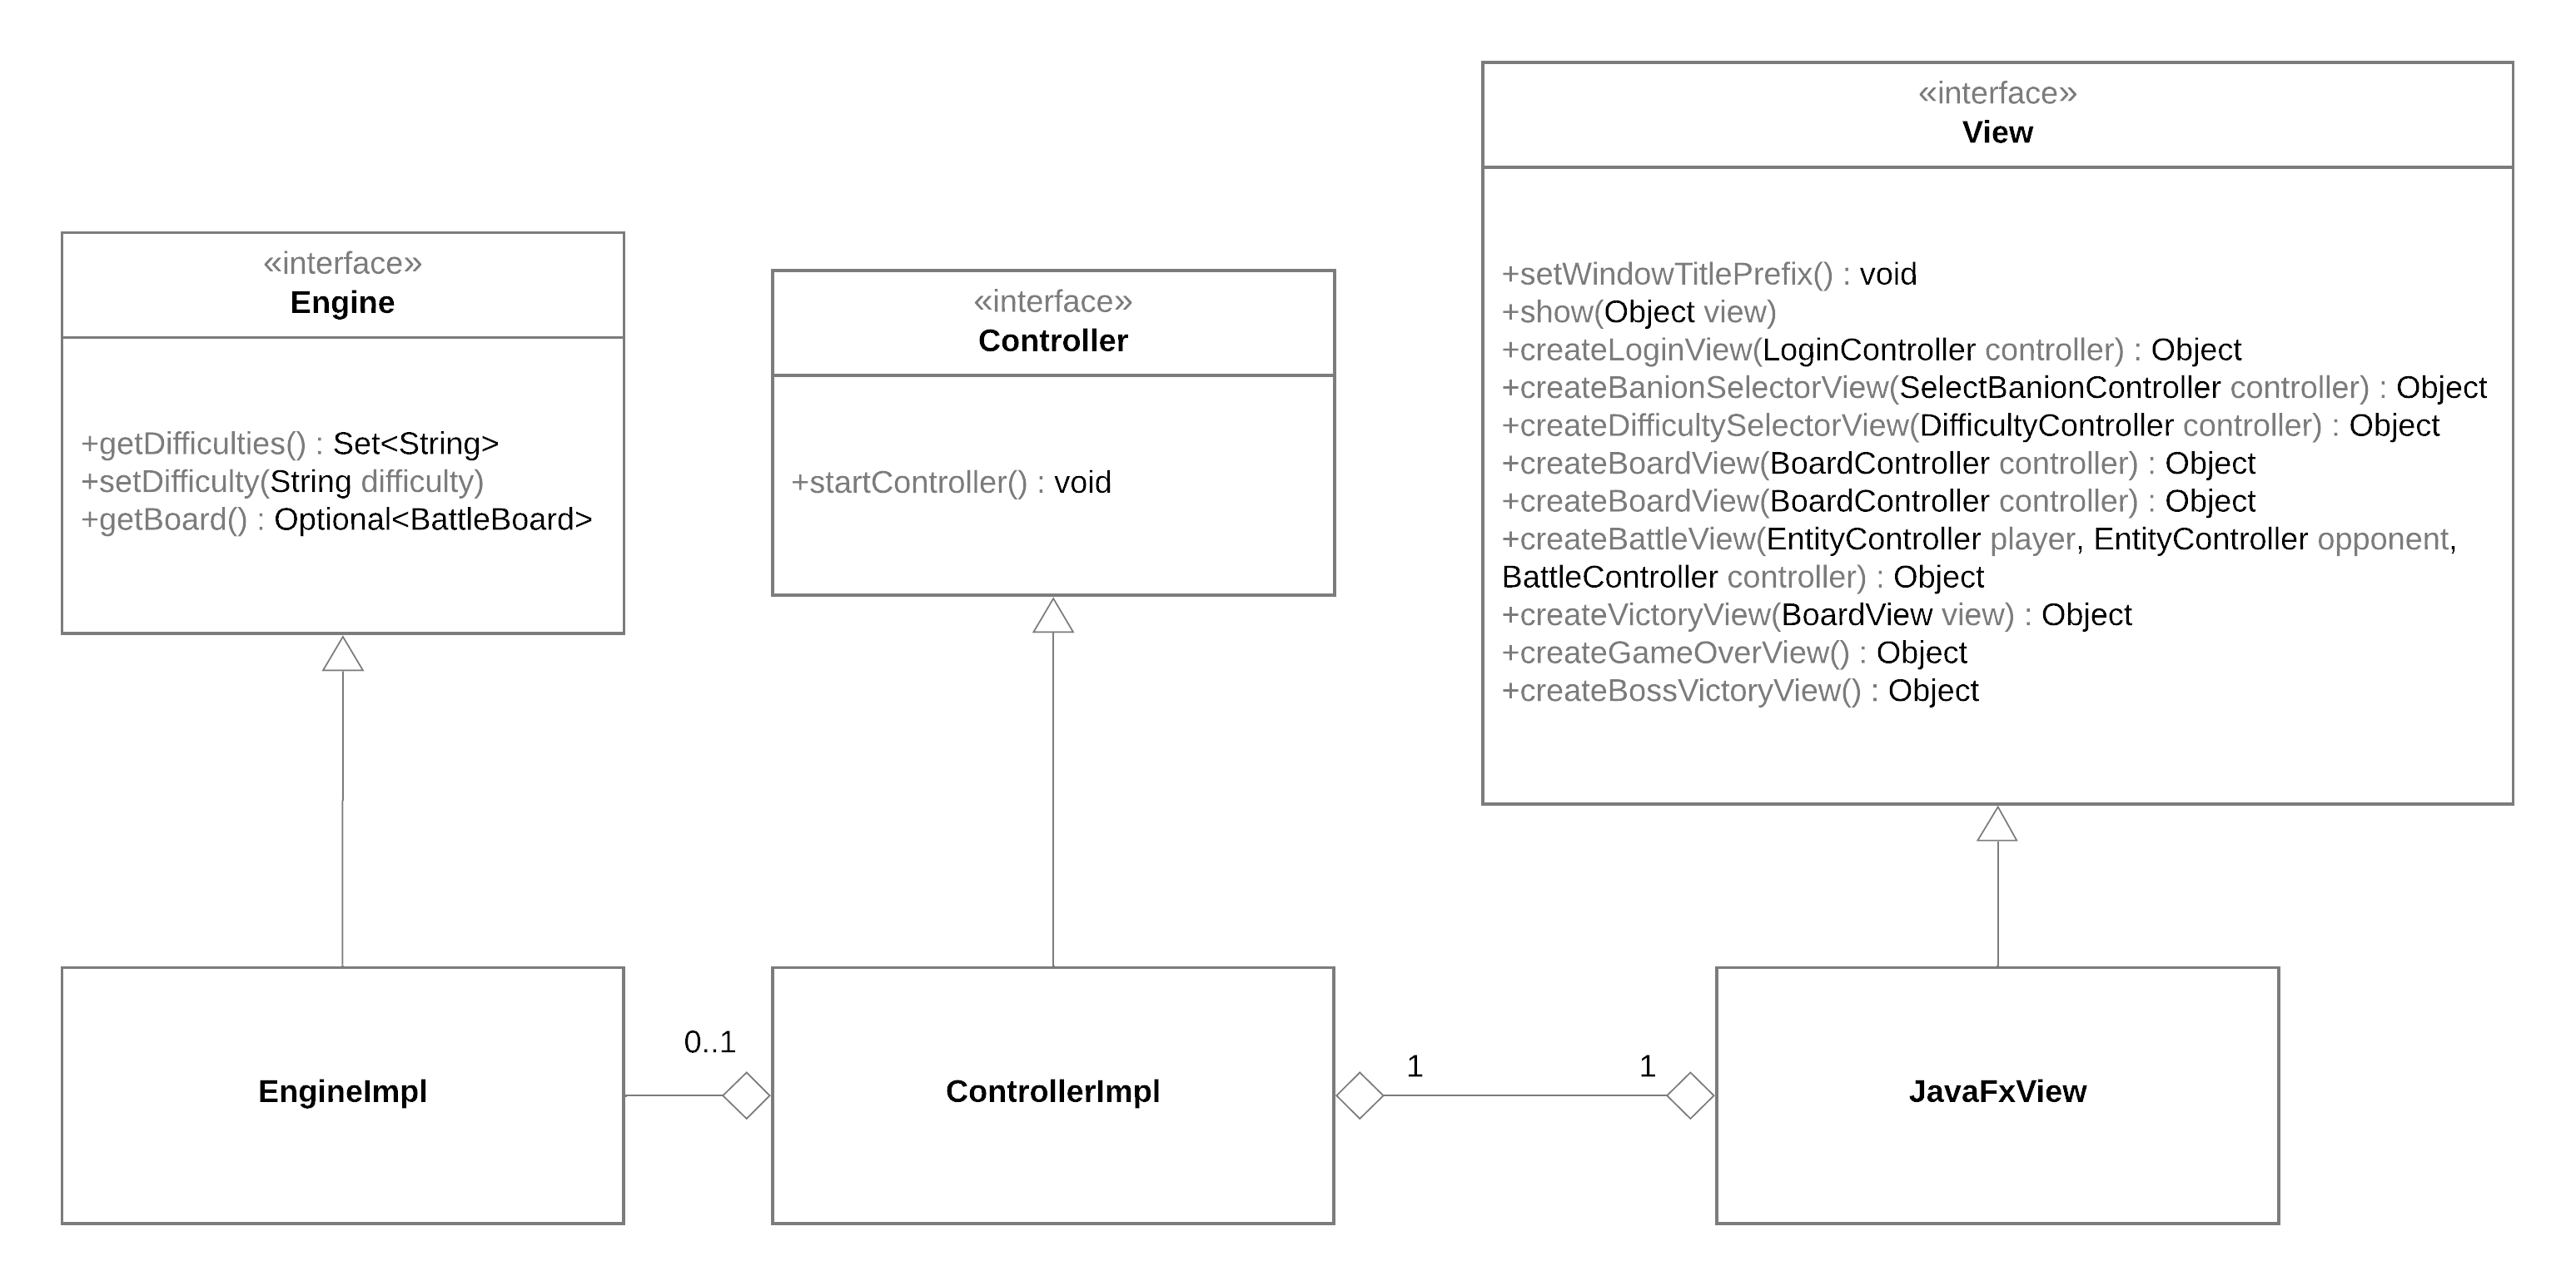
\includegraphics[width=12cm]{mvc}
    \caption{UML Model-View-Controller}
    \end{figure}

\section{Details}

    \subsection*{Enrico Marchionni}

        \subsubsection{Game Difficulty}

            \paragraph{Problem}
            
            Giving the possibility to choose between different thought games.
            Each difficulty should determine for example the number of tiles for the \emph{Board}, the moving \emph{Strategy} in it,
            the number and \emph{Element} of the \emph{Opponent}'s \emph{Banion}s, the \emph{AI} for each \emph{Opponent}...
            A requirement is that this problem has to be resolved in an extendible way.
            So once the system is built, adding a difficulty must be easy and fast according to \emph{OCP} (open closed principle).

            \paragraph{Solution}

            The element \emph{Board} is the main entity of this game because it determines how much
            levels have to be completed to win the game. So the main \emph{Model} class that is responsible for
            the difficulties is the \emph{Engine} class. It retrieves the \emph{Board} and everything else go by itself
            only by selecting the \emph{Difficulty}. The difficulty has the goal to decide the \emph{Board} \emph{Strategy} of
            movement, the number of levels and the \emph{AI} associated with the \emph{Opponent}. Each \emph{Opponent} will
            be created by the \emph{Board} at the right moment through an \emph{OpponentFactory} that was created by the \emph{Difficulty}
            itself.

            \begin{figure}[ht]
            \centering{}
            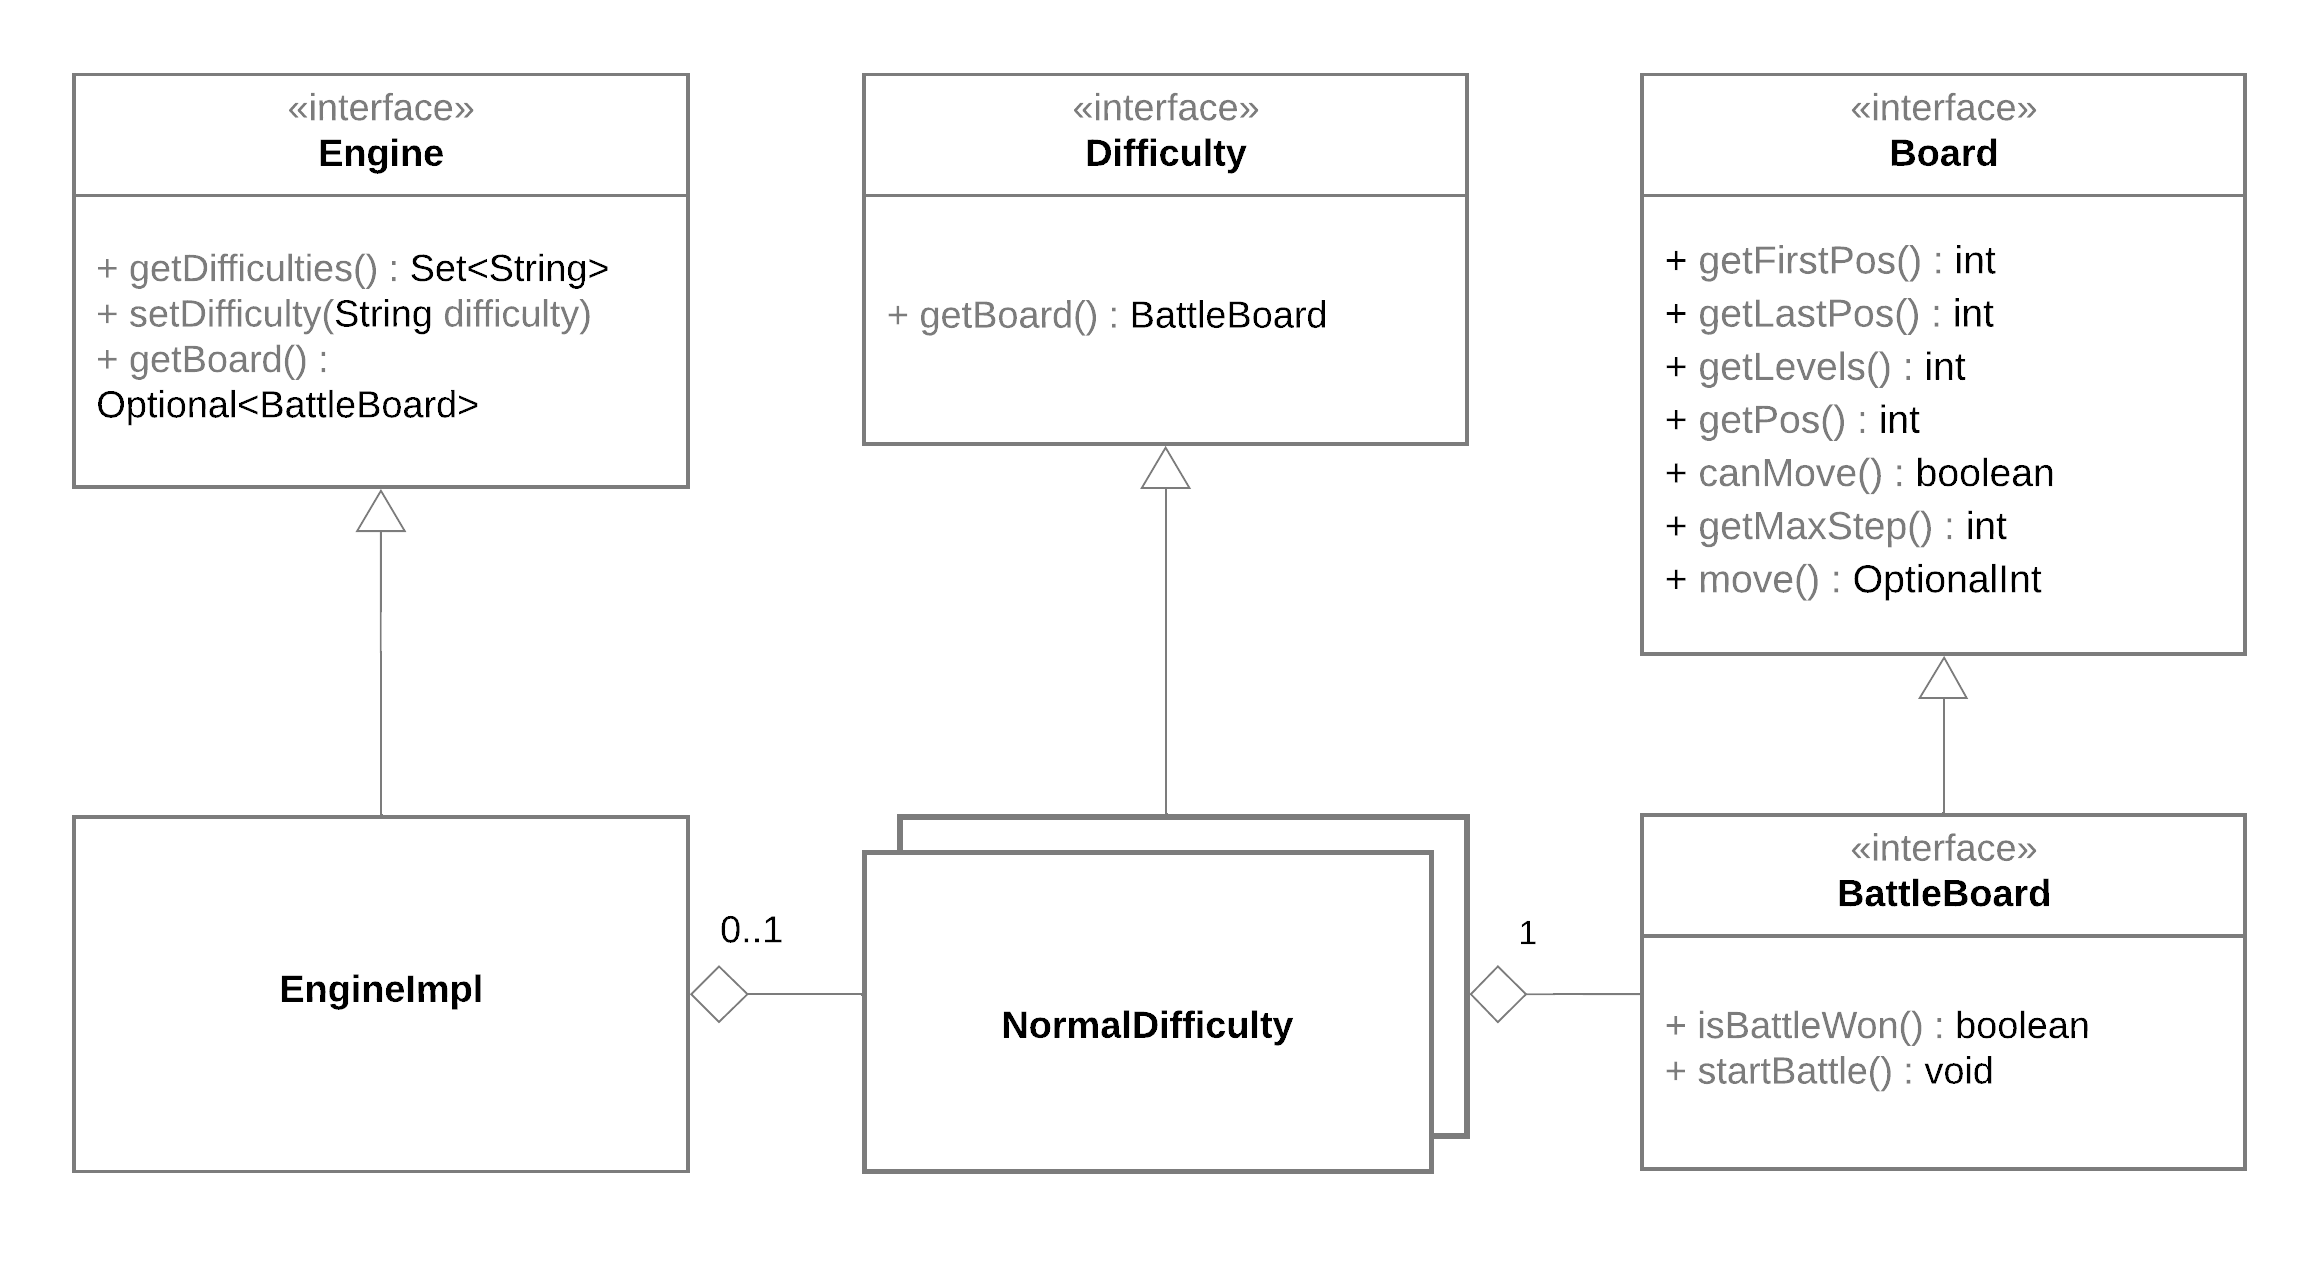
\includegraphics[width=\textwidth]{difficulty}
            \caption{UML difficulty}
            % \label{img:difficulty}
            % \ref{img:difficulty}
            \end{figure}

            \paragraph{Pattern}

            The \emph{Difficulty} decides the \emph{Board} step of movement by passing a \emph{PositiveIntSupplier} to \emph{Board} constructor via \emph{Strategy}.
            Furthermore the \emph{Difficulty} decides also the \emph{OpponentFactory} implementation to pass to the \emph{Board} via \emph{Strategy}.
            The \emph{OpponentFactory} can be considered as \emph{Abstract Factory} because every single implementation of \emph{Difficulty} could pass
            a different implementation of \emph{OpponentFactory} to the relative \emph{BattleBoard}.

        \subsubsection{\emph{Banion}}

            \paragraph{Problem}

            We wanted to make two \emph{Banion}s with same name and statistics be considered different at \emph{Domain Model} level.

            \paragraph{Solution}

            After evaluating different options such as not overriding \emph{Banion}'s equals, we decided to use
            \href{https://docs.oracle.com/en/java/javase/17/docs/api/java.base/java/util/UUID.html}{\textit{java.util.UUID}} class to identify every single \emph{Banion} instance.
            In this way it is possible for a player for example to have in the inventory two \emph{Banion}s with the same name twice, because they are different.

        \subsubsection{\emph{Element}s, \emph{Move}s and \emph{Banion}s Generation}

            \paragraph{Problem}
            
            Generating game entities: \emph{Element}, \emph{Move} and \emph{Banion}. Our game needs a consistent number of \emph{Banion}s \ref{table:banions} to be playable.
            It would better if they could be the same every time the application starts: same names, same sprites, same moves...
            Independently from the user progresses it would be nice for a user to choose between the same set of Banions at the beginning of every new the game.

            \paragraph{Solution}

            The problem is that somehow these entities has to be created, so how I decided to do that is the solution.
            At the beginning I started from the generation of \emph{Element}s \ref{table:elements} by coding each one in Java classes.
            The two main problems I observed were the expansion of classes and the inability to easily and quickly add new ones.
            After that I took time to think at a more extendible and cleaner solution, at the end I decided to go for the deserialization.
            I decided to create in the MVC \emph{Controller} a system to deserialize entities from file.
            In specific I chose \textit{.json}, using \href{https://github.com/google/gson}{Google Gson} library.
            
            I also wanted to make sure to avoid duplication of information.
            We decided that every single entity must be identifiable by name.
            So I created three files, one for each entity to generate, following this structure:
            \begin{itemize}
                \item \emph{Element} \textrightarrow independent from the other entities;
                \item \emph{Move} \textrightarrow dependent from \emph{Element} entities (each \emph{Move} is associated with one \emph{Element});
                \item \emph{Banion} \textrightarrow dependent from \emph{Element} and \emph{Move} entities (each \emph{Banion} is associated with one \emph{Element} and 4 \emph{Move}s);
            \end{itemize}

            I also decoupled file reading from entities generation.
            I put in the \textit{darwinsquest.config} package classes to read from file while in \textit{darwinsquest.config} I put the Factories according to \emph{SRP} (single responsibility principle).

            \paragraph{Pattern}

            The entities are created by using \emph{Abstract Factory} pattern.
            \emph{ElementFactory}, \emph{MoveFactory} and \emph{BanionFactory} retrieves the deserialized data with the shape of a set.

            \paragraph{Comments}

            Following this scheme in future it could be easily add the functionality of writing a system to save user progress.
            This would consist essentially on storing user \emph{Banion}s data in a folder (ex. \emph{.darwinsquest} in the user folder) and reload them after the login operation.
            For what concerns \emph{User} and \emph{Board} progresses serialization it should be thought in organization, and it would be integrated with the serialization/deserialization of entities.

        \subsubsection{\emph{Sprite}s}

            \paragraph{Problem}

            Each \emph{Banion} should be represented by a \emph{Sprite} in the \emph{View}.

            \paragraph{Solution}

            I considered that each \emph{Banion} is uniquely identified by its name.
            So I decided to put the necessary data in the same \textit{.json} file that contained also the \emph{Banion}s information.
            By doing that I created a \emph{BanionsSpriteFactory} class in the \emph{View} that has to read \emph{Sprite} record (it contains \emph{Banion} .png information).
            Each banion will be associated in the \emph{View} to its \emph{Sprite} by its name (this can be seen in \emph{ChooseBanionMenuView} constructor).

        \subsubsection{View}

            \paragraph{Problem}

            How to separate concerns in the chosen \emph{JavaFX} library.
            How to decouple style from showing controls, for example how to specify each \emph{Scene} font in a \emph{DRY} (don't repeat yourself) way.

            \paragraph{Solution}

            I started by using \textit{.css} files to specify style and \textit{.fxml} to specify layouts for each Container.
            I created a Controller for each Container.
            I created a \textit{View} interface that is a generic interface with the aim to create and show different views.
            In this way the \textit{View} interface remains generic and could potentially change without modifying its interfaces.

    \subsection*{Francesco Cipollone}

    \dots

    \subsection*{Raffaele Marrazzo}

    \dots

\chapter{Deployment}

\section{Automatized testing}

    We used \emph{JUnit} to test our \emph{Model} classes.

    \subsection*{Enrico Marchionni}

    \subsubsection{TestNormalDifficulty}
    
    Tests difficulty and opponents factory behavior;

    \subsubsection{TestBanion}
    
    Tests if \emph{Banion} behaves correctly, and if \emph{Element}s are correctly related to \emph{Banion}s;

    \subsubsection{TestEngine}
    
    Tests \emph{Engine} behavior as difficulty provider.

    \subsubsection{TestAssert}
    
    Despite using additional libraries such as \href{https://commons.apache.org/proper/commons-lang/}{apache commons-lang3}
    I implemented the utility \emph{darwinsquest.util.Asserts} class to accelerate arguments checks in a fluently way.

    \subsubsection{TestCollectors}
    
    Tests the \emph{darwinsquest.util.Collectors} utility class necessary to collect data to an immutable view of \emph{java.util.LinkedHashSet} for example.

    \subsubsection{TestGeneration}
    
    Tests the correct generation of entities, how described in my \emph{Details} section.

    \subsubsection{View}

    For questions of time and lack of knowledge I wasn't able to test the \emph{View}.

    \subsection*{Francesco Cipollone}

    \dots

    \subsection*{Raffaele Marrazzo}

    \dots

\section{Work strategy}

    We followed our \emph{Analysis} idea by developing the \emph{Model} main interfaces and classes.
    During development, we tried to adopt git-flow by creating a \emph{develop} branch and a new branch for each new \emph{feature}.

    ... problems with battle controller ...

    We proceeded as follows:

    \subsection*{Enrico Marchionni}

    \begin{itemize}
        \item Engine and Board;
        \item Game difficulties;
        \item Entities generation;
        \item JavaFX \emph{View} controllers of start menu, login, difficulties selector, board, choose banions selector, and JavaFXView class;
        \item Main controller class;
    \end{itemize}

    \subsection*{Francesco Cipollone}

    \dots

    \subsection*{Raffaele Marrazzo}

    \dots

\section{Development notes}

    Each one of us used these advanced aspects of language:

    \subsection*{Enrico Marchionni}

        \subsubsection{Bounded type parameters}

        Used in a few occasions.

        Example at \url{https://github.com/DarwinsQuest/DarwinsQuest/blob/3ec97da07e9622ab8ec0333a774619be3332e88e/src/main/java/darwinsquest/util/EObserver.java#L15}.

        \subsubsection{Generic class}
        
        Used frequently.

        Example at \url{https://github.com/DarwinsQuest/DarwinsQuest/blob/3ec97da07e9622ab8ec0333a774619be3332e88e/src/main/java/darwinsquest/config/CustomDeserializer.java#L47}.

        \subsubsection{Annotation \emph{darwinsquest.annotation.Description}}

        I used this custom annotations in 2 different scopes.

        Example 1 at \url{https://github.com/DarwinsQuest/DarwinsQuest/blob/3ec97da07e9622ab8ec0333a774619be3332e88e/src/main/java/darwinsquest/core/EngineImpl.java#L38}.

        Example 2 at \url{https://github.com/DarwinsQuest/DarwinsQuest/blob/3ec97da07e9622ab8ec0333a774619be3332e88e/src/main/java/darwinsquest/view/JavaFXView.java#L56}.

        \subsubsection{Reflection}

        Used in different situations.

        Example at \url{https://github.com/DarwinsQuest/DarwinsQuest/blob/3ec97da07e9622ab8ec0333a774619be3332e88e/src/main/java/darwinsquest/core/EngineImpl.java#L65}.

        \subsubsection{Lambda expressions}

        Used very frequently.

        Example at \url{https://github.com/DarwinsQuest/DarwinsQuest/blob/3ec97da07e9622ab8ec0333a774619be3332e88e/src/main/java/darwinsquest/core/gameobject/banion/BanionImpl.java#L57}.

        \subsubsection{Optional}

        Used very frequently.

        Example at \url{https://github.com/DarwinsQuest/DarwinsQuest/blob/3ec97da07e9622ab8ec0333a774619be3332e88e/src/main/java/darwinsquest/core/Engine.java#L31}.

        \subsubsection{Stream}

        Used very frequently.

        Example at \url{https://github.com/DarwinsQuest/DarwinsQuest/blob/3ec97da07e9622ab8ec0333a774619be3332e88e/src/main/java/darwinsquest/view/ChooseBanionMenuView.java#L69}.

        \subsubsection{Immutable ordered set}

        Used only at \url{https://github.com/DarwinsQuest/DarwinsQuest/blob/3ec97da07e9622ab8ec0333a774619be3332e88e/src/main/java/darwinsquest/core/EngineImpl.java#L46}.

        \subsubsection{Library \href{https://openjfx.io/}{JavaFX}}
        
        Used for \emph{View} management.

        Example at \textit{fxml} with \textit{.css}, example at \url{https://github.com/DarwinsQuest/DarwinsQuest/blob/3ec97da07e9622ab8ec0333a774619be3332e88e/src/main/java/darwinsquest/view/JavaFXView.java#L53}.
        
        \subsubsection{Library \href{https://commons.apache.org/proper/commons-lang/}{Apache Commons Lang 3}}
        
        Used frequently.

        Example at \url{https://github.com/DarwinsQuest/DarwinsQuest/blob/3ec97da07e9622ab8ec0333a774619be3332e88e/src/main/java/darwinsquest/view/graphics/BanionsSpriteFactory.java#L27}.
        
        \subsubsection{Library \href{https://github.com/google/gson}{Google Gson}}
        
        Used for deserialization.

        Example at \url{https://github.com/DarwinsQuest/DarwinsQuest/blob/3ec97da07e9622ab8ec0333a774619be3332e88e/src/main/java/darwinsquest/util/JsonUtils.java#L81}.
        
        \subsubsection{Library \href{https://github.com/DiUS/java-faker}{Java Faker}}
        
        Used only at \url{https://github.com/DarwinsQuest/DarwinsQuest/blob/3ec97da07e9622ab8ec0333a774619be3332e88e/src/main/java/darwinsquest/core/difficulty/OpponentsFactoryImpl.java#L114}.

    \subsection*{Francesco Cipollone}

    \dots

    \subsection*{Raffaele Marrazzo}

    \dots

\chapter{Final comments}

    Tile concept was never used in our battle \emph{Board} that consists in a series of battles that can be skipped by die jump.
    It would be better to introduce different \emph{Tile}s and to be forced to complete \emph{BattleTile}s, while the others can be skipped.

\section{Self-evaluation and future improvements}

    \subsection*{Enrico Marchionni}
    
    \dots

    \subsection*{Francesco Cipollone}

    \dots

    \subsection*{Raffaele Marrazzo}

    \dots

\section{Difficulties and comments to teachers}

    \subsection*{Francesco Cipollone}

    \dots

    \subsection*{Raffaele Marrazzo}

    \dots

\appendix

\chapter{User guide}

    \dots

\chapter{Laboratory}

\section{enrico.marchionni@studio.unibo.it}

\begin{itemize}
    \item Lab 04: \url{https://virtuale.unibo.it/mod/forum/discuss.php?d=113869#p169173}
    \item Lab 05: \url{https://virtuale.unibo.it/mod/forum/discuss.php?d=114647#p169723}
    \item Lab 06: \url{https://virtuale.unibo.it/mod/forum/discuss.php?d=115548#p171159}
    \item Lab 07: \url{https://virtuale.unibo.it/mod/forum/discuss.php?d=117044#p173058}
    \item Lab 08: \url{https://virtuale.unibo.it/mod/forum/discuss.php?d=117852#p174127}
    \item Lab 09: \url{https://virtuale.unibo.it/mod/forum/discuss.php?d=118995#p175326}
    \item Lab 10: \url{https://virtuale.unibo.it/mod/forum/discuss.php?d=119938#p176522}
    \item Lab 11: \url{https://virtuale.unibo.it/mod/forum/discuss.php?d=121130#p177368}
    \item Lab 12: \url{https://virtuale.unibo.it/mod/forum/discuss.php?d=121885#p178425}
\end{itemize}

\printbibliography

\end{document}